% Scratch file for iterating on the FourierBGC encoding zoom-in figure.
%   pdflatex fourierbgc_encoding_diagram.tex

\documentclass[tikz,border=8pt]{standalone}
\usepackage{amsmath}
\usetikzlibrary{positioning,fit,backgrounds,calc,arrows.meta,decorations.pathreplacing}

\begin{document}
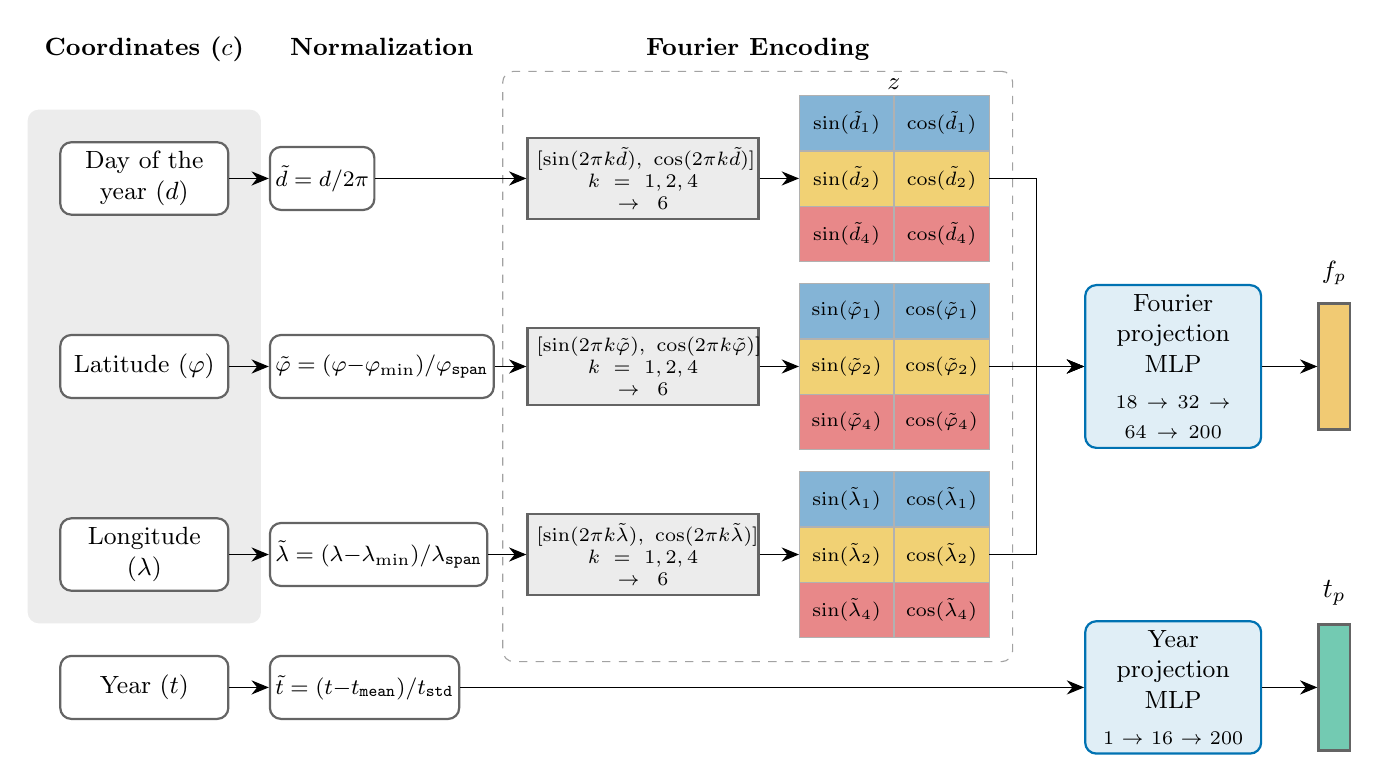
\begin{tikzpicture}[
  font=\small,
  >={Stealth[length=2.2mm,width=1.8mm]},
  node distance=3mm and 5mm,
]

\definecolor{coordcolor}{RGB}{230,159,0}
\definecolor{profcolor}{RGB}{0,158,115}
\definecolor{rule}{RGB}{100,100,100}
\definecolor{enccolor}{RGB}{0,114,178}
\definecolor{k1color}{RGB}{31,119,180}
\definecolor{k2color}{RGB}{230,171,2}
\definecolor{k4color}{RGB}{214,39,40}

\tikzstyle{inputbox} = [draw=rule, thick, rounded corners, fill=white, align=center, minimum height=8mm, text width=19mm, font=\small]
\tikzstyle{normbox}  = [draw=rule, thick, rounded corners, align=center, minimum height=8mm, inner sep=2pt, font=\footnotesize\ttfamily]
\tikzstyle{eqbox}    = [draw=rule, thick, fill=rule!12, align=center, minimum height=9mm, text width=27mm, font=\scriptsize]
\tikzstyle{mlpbox}   = [draw=enccolor, thick, fill=enccolor!12, rounded corners, align=center, minimum height=16mm, text width=20mm]
\tikzstyle{outbar}   = [draw=rule, thick, fill=coordcolor!55, minimum width=4mm, minimum height=16mm]
\tikzstyle{grouplabel} = [font=\bfseries\small, text=black]
\tikzstyle{gridcell} = [draw=rule!50, very thin, minimum width=12mm, minimum height=7mm, font=\scriptsize, align=center, inner sep=0pt]

\node[inputbox] (d-in) {Day of the year ($d$)};
\node[normbox, right=of d-in] (d-norm) {$\tilde{d} = d/2\pi$};

\node[inputbox, below=15mm of d-in] (phi-in) {Latitude ($\varphi$)};
\node[normbox, right=of phi-in] (phi-norm)
  {$\tilde{\varphi} = (\varphi{-}\varphi_{\min})/\varphi_{\text{span}}$};

\node[inputbox, below=15mm of phi-in] (lam-in) {Longitude ($\lambda$)};
\node[normbox, right=of lam-in] (lam-norm)
  {$\tilde{\lambda} = (\lambda{-}\lambda_{\min})/\lambda_{\text{span}}$};

\coordinate (eqcol) at ($(phi-norm.east)+(4mm,0)$);

\node[eqbox, anchor=west] (d-eq) at (eqcol |- d-in)
  {$[\sin(2\pi k\tilde{d}),\ \cos(2\pi k\tilde{d})]$ \\ \scriptsize $k=1,2,4$ \\ $\rightarrow 6$};
\node[eqbox, anchor=west] (phi-eq) at (eqcol |- phi-norm)
  {$[\sin(2\pi k\tilde{\varphi}),\ \cos(2\pi k\tilde{\varphi})]$ \\ \scriptsize $k=1,2,4$ \\ $\rightarrow 6$};
\node[eqbox, anchor=west] (lam-eq) at (eqcol |- lam-norm)
  {$[\sin(2\pi k\tilde{\lambda}),\ \cos(2\pi k\tilde{\lambda})]$ \\ \scriptsize $k=1,2,4$ \\ $\rightarrow 6$};

\node[gridcell, fill=k2color!55, right=5mm of d-eq] (d-blk2-sin) {$\sin(\tilde{d}_2)$};
\node[gridcell, fill=k2color!55, right=0mm of d-blk2-sin] (d-blk2-cos) {$\cos(\tilde{d}_2)$};
\node[gridcell, fill=k1color!55, above=0mm of d-blk2-sin] (d-blk1-sin) {$\sin(\tilde{d}_1)$};
\node[gridcell, fill=k1color!55, right=0mm of d-blk1-sin] (d-blk1-cos) {$\cos(\tilde{d}_1)$};
\node[gridcell, fill=k4color!55, below=0mm of d-blk2-sin] (d-blk4-sin) {$\sin(\tilde{d}_4)$};
\node[gridcell, fill=k4color!55, right=0mm of d-blk4-sin] (d-blk4-cos) {$\cos(\tilde{d}_4)$};

\node[coordinate] (topline) at ($(d-blk1-sin.north)+(0,5mm)$) {};

\node[gridcell, fill=k2color!55, right=5mm of phi-eq] (phi-blk2-sin) {$\sin(\tilde{\varphi}_2)$};
\node[gridcell, fill=k2color!55, right=0mm of phi-blk2-sin] (phi-blk2-cos) {$\cos(\tilde{\varphi}_2)$};
\node[gridcell, fill=k1color!55, above=0mm of phi-blk2-sin] (phi-blk1-sin) {$\sin(\tilde{\varphi}_1)$};
\node[gridcell, fill=k1color!55, right=0mm of phi-blk1-sin] (phi-blk1-cos) {$\cos(\tilde{\varphi}_1)$};
\node[gridcell, fill=k4color!55, below=0mm of phi-blk2-sin] (phi-blk4-sin) {$\sin(\tilde{\varphi}_4)$};
\node[gridcell, fill=k4color!55, right=0mm of phi-blk4-sin] (phi-blk4-cos) {$\cos(\tilde{\varphi}_4)$};

\node[gridcell, fill=k2color!55, right=5mm of lam-eq] (lam-blk2-sin) {$\sin(\tilde{\lambda}_2)$};
\node[gridcell, fill=k2color!55, right=0mm of lam-blk2-sin] (lam-blk2-cos) {$\cos(\tilde{\lambda}_2)$};
\node[gridcell, fill=k1color!55, above=0mm of lam-blk2-sin] (lam-blk1-sin) {$\sin(\tilde{\lambda}_1)$};
\node[gridcell, fill=k1color!55, right=0mm of lam-blk1-sin] (lam-blk1-cos) {$\cos(\tilde{\lambda}_1)$};
\node[gridcell, fill=k4color!55, below=0mm of lam-blk2-sin] (lam-blk4-sin) {$\sin(\tilde{\lambda}_4)$};
\node[gridcell, fill=k4color!55, right=0mm of lam-blk4-sin] (lam-blk4-cos) {$\cos(\tilde{\lambda}_4)$};

\begin{scope}[on background layer]
  \node[fill=rule!12, rounded corners, inner sep=4mm,
        fit=(d-in)(phi-in)(lam-in)] (coord-wrap) {};
\end{scope}
\begin{scope}[on background layer]
  \node[draw=rule!60, dashed, rounded corners, inner sep=3mm,
        fit=(d-eq)(d-blk1-sin)(d-blk4-cos)
            (phi-eq)(phi-blk1-sin)(phi-blk4-cos)
            (lam-eq)(lam-blk1-sin)(lam-blk4-cos)] (fourier-wrap) {};
\end{scope}

\node[grouplabel, anchor=base] at (coord-wrap.center |- topline) {Coordinates ($c$)};
\node[grouplabel, anchor=base] at (phi-norm.center |- topline) {Normalization};
\node[grouplabel, anchor=base] at (fourier-wrap.center |- topline) {Fourier Encoding};

\draw[->] (d-in) -- (d-norm);
\draw[->] (d-norm) -- (d-eq);
\draw[->] (d-eq) -- (d-blk2-sin.west|-d-eq);

\draw[->] (phi-in) -- (phi-norm);
\draw[->] (phi-norm) -- (phi-eq);
\draw[->] (phi-eq) -- (phi-blk2-sin.west|-phi-eq);

\draw[->] (lam-in) -- (lam-norm);
\draw[->] (lam-norm) -- (lam-eq);
\draw[->] (lam-eq) -- (lam-blk2-sin.west|-lam-eq);

\node[mlpbox, anchor=west] (mlp) at ($(fourier-wrap.east |- phi-blk2-sin)+(9mm,0)$)
  {Fourier\\projection\\MLP\\[2pt]\scriptsize $18\to32\to64\to200$};

\coordinate (mergeX) at ($(fourier-wrap.east)+(3mm,0)$);
\coordinate (d-out) at (d-blk2-cos.east);
\coordinate (phi-out) at (phi-blk2-cos.east);
\coordinate (lam-out) at (lam-blk2-cos.east);
\draw[->] (d-out) -- (mergeX |- d-out) |- (mlp.west);
\draw[->] (phi-out) -- (mlp.west);
\draw[->] (lam-out) -- (mergeX |- lam-out) |- (mlp.west);

\node[outbar, right=7mm of mlp] (fp) {};
\node[above=1mm of fp, font=\fontsize{9}{11}\selectfont] {$f_p$};
\draw[->] (mlp) -- (fp);

\node[inputbox, below=8mm of lam-in] (year-in) {Year ($t$)};
\node[normbox, right=of year-in] (year-norm)
  {$\tilde{t} = (t{-}t_{\text{mean}})/t_{\text{std}}$};
\node[mlpbox] (year-mlp) at (mlp |- year-in)
  {Year\\projection\\MLP\\[2pt]\scriptsize $1\to16\to200$};
\node[outbar, fill=profcolor!55] (tp) at (fp |- year-in) {};
\node[above=1mm of tp, font=\fontsize{10}{11}\selectfont] {$t_p$};
\draw[->] (year-in) -- (year-norm);
\draw[->] (year-norm) -- (year-mlp);
\draw[->] (year-mlp) -- (tp);
\node at (9.52,1.20) {$z$};
\end{tikzpicture}
\end{document}
